\section{SPH 方法回顾}

\subsection{光滑核函数插值}

\begin{frame}
    一个物理场量 $A(\vec{r})$ 可以用其在空间中分布的加权积分得到:
    \begin{equation}
        A(\vec{r}) = \int A(\vec{r}^\prime) W(\vec{r} - \vec{r}^\prime, h) \mathrm{d} \vec{r}^\prime
    \end{equation}
    其中 $W(\vec{r} - \vec{r}^\prime, h)$ 是光滑核函数,$h$ 是光滑长度。
    这是一个与 $\delta(\vec{r})$ 相似的函数,但是具有有限的支撑域。
    一个物理量的核函数插值,仅由其在支撑域内的物理量决定。
    同时,该物理量梯度经分部积分和边界舍入,也可以表达为:
    \begin{equation}
        \nabla A(\vec{r}) = \int A(\vec{r}^\prime) \nabla W(\vec{r} - \vec{r}^\prime, h) \mathrm{d} \vec{r}^\prime
    \end{equation}
    在物理量被一颗颗粒子携带的时候,
    上述积分可以表示为对支撑域内所有粒子的加权求和:
    \begin{equation}
        \begin{aligned}
            A_i &= \sum_j \frac{m_j}{\rho_j} A_j W_{ij} \\
            \nabla A_i &= \sum_j \frac{m_j}{\rho_j} A_j \nabla W_{ij}
        \end{aligned}
    \end{equation}
\end{frame}

\begin{frame}
    如下图为目前实现的四个光滑核函数在光滑核半径为 $0.1$ 时的值。
    \begin{figure}[H]
        \centering
        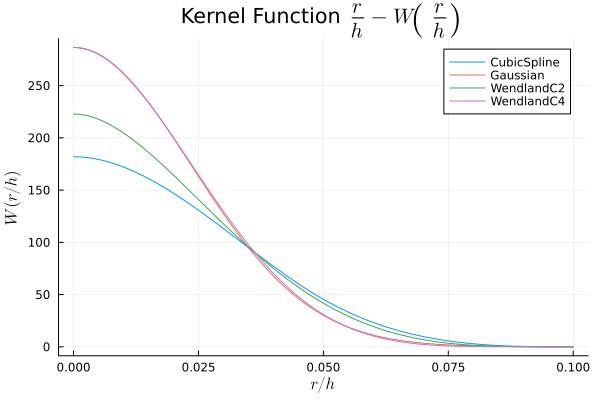
\includegraphics[width=0.9\textwidth]{images/kernel_value.png}
        \caption{光滑核函数的值}
    \end{figure}
\end{frame}

\begin{frame}
    记 $q=\frac{r}{h}$,则 $\vec{\nabla} W$ 的表达式为:
    \begin{equation}
        \begin{aligned}
            \vec{\nabla} W 
            &= \vec{e}_i\frac{\partial}{\partial x_i}W\left(\frac{r}{h}\right)\\
            &= W^\prime(q)\frac{1}{h}\vec{e}_i\frac{\partial r}{\partial x_i}\\
            &= \frac{1}{h}W^\prime(q) \frac{x_i}{r}\vec{e}_i\\
        \end{aligned}
    \end{equation}
    其中 $W^\prime(q)$ 为光滑核函数关于相对半径 $q$ 的导数。
    可以发现光滑核函数的梯度与 $x_i\vec{e}_i$ 有着一致的方向,且:
    \begin{equation}
        |\vec{\nabla}W| = \left|\frac{1}{h}W^\prime(q)\right|
    \end{equation}
\end{frame}

\begin{frame}
    如下图为目前实现的四个光滑核函数的 $\frac{1}{h}W^\prime(q)$ 在光滑核半径为 $0.1$ 时的值。
    可以发现 $W^\prime(q)$ 恒负,该结果我和开源库比较过,是一致的。
    \begin{figure}[H]
        \centering
        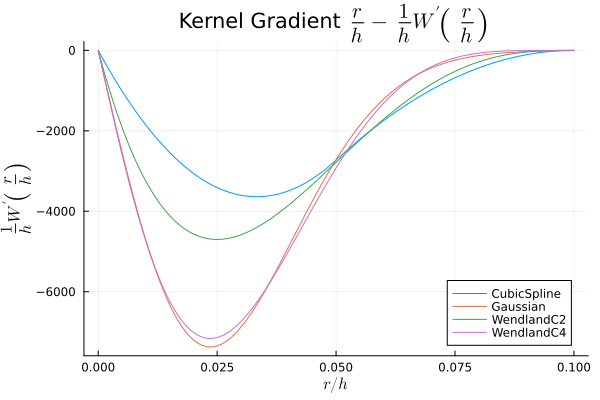
\includegraphics[width=0.9\textwidth]{images/kernel_gradient.png}
        \caption{光滑核函数的梯度值}
    \end{figure}
\end{frame}

\subsection{SPH 方法的基本方程}

\begin{frame}
    在 Lagrange 描述下,不可压流体的基本方程为,
    暂时不考虑能量方程。
    \begin{equation}
        \begin{aligned}
            \frac{\mathrm{d} \rho}{\mathrm{d} t} &= -\rho \nabla \cdot \vec{v} \\
            \frac{\mathrm{d} \vec{v}}{\mathrm{d} t} &= -\frac{1}{\rho} \nabla p + \vec{g} + \nu \nabla^2 \vec{v}\\
            \frac{\mathrm{d} \vec{x}}{\mathrm{d} t} &= \vec{v}
        \end{aligned}
    \end{equation}
    目前 SPH 方法广为使用的方式是弱可压 WCSPH 方法,
    其允许流体的密度在一定范围内变化。
    并且给出了状态方程如下:
    \begin{equation}
        p = \frac{c_0^2\rho_0}{\gamma}
        \left[\left(\frac{\rho}{\rho_0}\right)^\gamma - 1\right]=
        \frac{c_0^2\rho_0}{\gamma}
        \left[\left(1+\frac{\rho-\rho_0}{\rho_0}\right)^\gamma - 1\right]
    \end{equation}
    在 $\rho$ 变化不大时,方程可以退化为 $p=c_0^2(\rho-\rho_0)$。
\end{frame}

\begin{frame}
    对于上述方程,
    我查阅了一些开源库和书籍论文,
    他们对于 $c_0$ 这个量的设定是“人工声速”。
    并非是真正的水的声速。
    而 $\gamma$ 一般设定为 $7$。
    可以推导在这种状态方程下,
    声速为:
    \begin{equation}
        c^2=\frac{\partial p}{\partial \rho}=c_0^2\left(\frac{\rho}{\rho_0}\right)^{\gamma - 1}
    \end{equation}
    而 $c_0$ 的值需要根据不同的算例设定不同的值来保证程序稳定性,
    一般取为:
    \begin{equation}
        c_0 = 10\max \{U_{\max}, \sqrt{g L_{\max}}\}
    \end{equation}
    这里的人工声速选取是我在程序内头痛的一个事情,我会在后续叙述。
\end{frame}

\subsection{SPH 方法的数值离散}

\begin{frame}
    根据光滑核函数插值,
    我们可以将 SPH 的控制方程离散成光滑核函数的插值形式:
    \begin{equation}
        \begin{aligned}
            \frac{\mathrm{d} \rho_i}{\mathrm{d} t} &= \rho_i \sum_j m_j \vec{v}_{ij} \cdot \nabla W_{ij} \\
            \frac{\mathrm{d} \vec{v}_i}{\mathrm{d} t} &= -\sum_j m_j \left(\frac{p_i}{\rho_i^2} + \frac{p_j}{\rho_j^2}\right) \nabla W_{ij} + \vec{g} + \nu \nabla^2 \vec{v}_i
        \end{aligned}
    \end{equation}
    其中粘性项的离散形式我没数学能力推导,
    直接采用了 SPHysics 开源库给出的形式如下:
    \begin{equation}
        \nu \nabla^2 \vec{v}_i = 
        \sum_j m_j
        \frac{4 (\mu_i + \mu_j) \vec{r}_{ij}\cdot \nabla W_{ij}}{(\rho_i + \rho_j)^2 (r_{ij}^2 + 0.01h^2)}\vec{v}_{ij}
    \end{equation}
\end{frame}